\section{Anomaly Detection}
\label{back:anomdet}

Anomaly detection, also referred to as outlier detection, is about identifying observations that can be deemed inconsistent with the rest of the dataset.  

Given the set $X = \{x_1, x_2, ..., x_n\}$, we define an anomaly as any sest of values $\theta_i$ in set $X$ such that $\theta_i - mean(X) > \epsilon$, where $\epsilon$ is a tresshold value. How one determine this value varies on a case by case scenario.

Anomaly detection can be performed in a lot of different ways. From common machine learning tasks such as K-means clustering \cite{7507933}, \Gls{svm} \cite{10.1007/978-3-540-28647-9_97}

Anomaly detection is used in a plethora of fields, such as networking, medical informatics and more. 

In essence, there are 3 main types of anomalies we'll be looking at. They are as follows:

\begin{enumerate}
    \item Point anomalies 
    \item Contextual anomalies 
    \item Collective anomalies
\end{enumerate}

While point anomalies target single instances that differ from the rest off the dataset, collective anomalies targets group of instances that together form an anomaly. Contextual ones, as in the word, require context to determine whether or not an anomaly has been detected. In the case of multichannel sensor data, collective anomalies become the most interesting ones. 


\subsection{Multivariate Anomaly detection}

In a one-dimensional time series, finding anomalies tend to be rather trivial. After taking neighbor values into account, look for sever outliers, .

Multivariate data analysis refers to statistical lookings from two or more variabels. In the case of sensor data, one often look at multiple sensors. 

Given a matrix $a$ of data:

\begin{equation}
\centering
\begin{matrix}
a_{11} &  0      & \ldots & a_{1n}    \\
0      &  a_{22} & \ldots & a_{2n}    \\
\vdots & \vdots  & \ddots & \vdots \\
a_{m1} &  0      &\ldots & a_{mn}
\end{matrix}
\caption{Matrix of data}
\end{equation}

We are interested in finding a region $a_{ij} to a_{kl}$ where $i < k \And j < l$ st. the values within these regions falls outside of the general range


For \acrshort{das} data specifically, anomaly detection can be used for detecting clusters of signals that don't correspond to the predisposed target feature. Registering these outlier signals and receiving real time information about these could prove vital in some cases,  and in best case scenario save lives. 

Dealing with sensitive data 

\subsection{Time series based anomaly detection}

Time series in one dimension is often a great candidate for anomaly detection. Stock market prediction, climate changes and several other series can be used to train networks to recognize point wise anomalies. Layers such as LSTM, RNN and GRU are constructed to store and retrieve information at a later time, thus introducing a memory mechanism. 

\subsection{Image based anomaly detection}

Anomaly detection can also be applied to images. Given a dataset of images with sheep, a image based anomaly detection model would be able to recognize any drastic changes between images. Without the temporal aspect of these problems, convolutional or linear layers are more often used. 

\begin{figure}[!h]
    \centering
    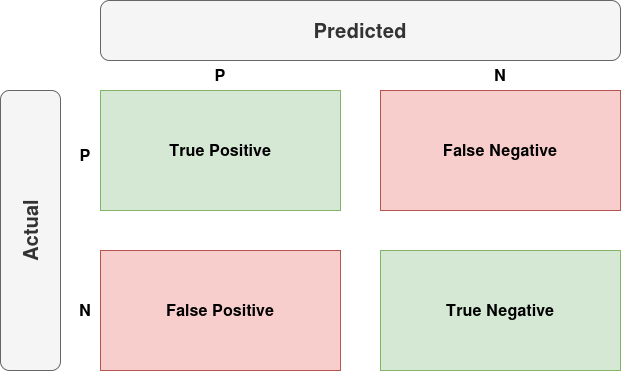
\includegraphics[width=0.5\linewidth]{figures/confmat.png}
    \caption{Caption}
    \label{fig:confmat}
\end{figure}
